\documentclass[wide,a4paper,titlepage,12pt] {article}
\usepackage{polski}
\usepackage[utf8]{inputenc}
\usepackage{listings}
\usepackage{slashbox}
\usepackage[table]{xcolor}
\usepackage{graphicx,pdflscape}
\usepackage{placeins}
\usepackage{slashbox}
\usepackage{longtable}


\title{Projektowanie efektywnych algorytmów}
\author{Tymon Tobolski (181037)\\ Jacek Wieczorek (181043)}

% Title page layout (fold)
\makeatletter
\renewcommand{\maketitle}{
\begin{titlepage}
  \begin{center}
    \vspace*{3cm}
    \LARGE \@title \par
    \vspace{2cm}
    \textit{\small Autor:}\par
    \normalsize \@author\par \normalsize
    \vspace{3cm}
    \textit{\small Prowadzący:}\par
   Prof. dr hab. inż Adam Janiak \par
    \vspace{2cm}
    Wydział Elektroniki\\ III rok\\ Cz TN 13.15 - 15.00\par
    \vspace{4cm}
    \small \@date
  \end{center}
\end{titlepage}
}
\makeatother

\begin{document}
\maketitle

\section{Cel projektu}
\paragraph{}
  Celem projektu jest zaimplementowanie i przetestowanie metaheurystycznego algorytmu genetycznego dla problemu szeregowania zadań na jednym procesorze przy kryterium minimalizacji ważonej sumy opóźnień zadań.

\section{Opis problemu}
{\bf Jednoprocesorowy problem szeregowania zadań przy kryterium
minimalizacji ważonej sumy opóźnień zadań.}

\paragraph{}
Danych jest $n$ zadań (o numerach od 1 do $n$), które mają być wykonane bez przerwań przez pojedynczy procesor, mogący wykonywać co najwyżej jedno zadanie jednocześnie.
Każde zadanie j jest dostępne do wykonania w chwili zero, do wykonania wymaga $p_{j} > 0$ jednostek czasu oraz ma określoną wagę (priorytet) $w_{j} > 0$ i oczekiwany termin zakończenia
wykonywania $d_{j} > 0$. Zadanie $j$ jest spóźnione, jeżeli zakończy się wykonywać po swoim terminie $d_{j}$, a miarą tego opóźnienia jest wielkość $T_{j} = max(0, C_{j} - d_{j} )$, gdzie $C_{j}$ jest terminem zakończenia
wykonywania zadania $j$. Problem polega na znalezieniu takiej kolejności wykonywania zadań (permutacji) aby zminimalizować kryterium $TWT = \Sigma_{j=1}^{n} w_{j} T_{j}$.

\section{Opis algorytmu}
\paragraph{}
Przebieg algorytmu :
\lstset{ %
    language=java,                % choose the language of the code
    basicstyle=\scriptsize,       % the size of the fonts that are used for the code
    numbers=left,                   % where to put the line-numbers
    numberstyle=\scriptsize,      % the size of the fonts that are used for the line-numbers
    stepnumber=10,                   % the step between two line-numbers. If it's 1 each line
                                    % will be numbered
    numbersep=9pt,                  % how far the line-numbers are from the code
    % backgroundcolor=\color{white},  % choose the background color. You must add \usepackage{color}
    showspaces=false,               % show spaces adding particular underscores
    showstringspaces=false,         % underline spaces within strings
    showtabs=false,                 % show tabs within strings adding particular underscores
    % frame=single,                 % adds a frame around the code
    % tabsize=2,                  % sets default tabsize to 2 spaces
    % captionpos=b,                   % sets the caption-position to bottom
    breaklines=true,                % sets automatic line breaking
    % breakatwhitespace=false,        % sets if automatic breaks should only happen at whitespace
    % title=\lstname,                 % show the filename of files included with \lstinputlisting;
                                    % also try caption instead of title
    % escapeinside={\%*}{*)},         % if you want to add a comment within your code
    % morekeywords={*,...}            % if you want to add more keywords to the set
    }
    \lstinputlisting{code/pseudokod.txt}
    \paragraph{}
    gdzie :
    \begin{itemize}
        \item F - funkcja kosztu/celu
        \item M - prawdopodobieństwo mutacji

    \end{itemize}

\section{Implementacja}
\paragraph{}
Jezykiem implementacji algorytmu jest $Scala$ w wersji $2.9.1$ działająca na $JVM$.
\paragraph{}
\lstset{ %
    language=java,                % choose the language of the code
    basicstyle=\scriptsize,       % the size of the fonts that are used for the code
    numbers=left,                   % where to put the line-numbers
    numberstyle=\scriptsize,      % the size of the fonts that are used for the line-numbers
    stepnumber=10,                   % the step between two line-numbers. If it's 1 each line
                                    % will be numbered
    numbersep=9pt,                  % how far the line-numbers are from the code
    % backgroundcolor=\color{white},  % choose the background color. You must add \usepackage{color}
    showspaces=false,               % show spaces adding particular underscores
    showstringspaces=false,         % underline spaces within strings
    showtabs=false,                 % show tabs within strings adding particular underscores
    % frame=single,                 % adds a frame around the code
    % tabsize=2,                  % sets default tabsize to 2 spaces
    % captionpos=b,                   % sets the caption-position to bottom
    breaklines=true,                % sets automatic line breaking
    % breakatwhitespace=false,        % sets if automatic breaks should only happen at whitespace
    % title=\lstname,                 % show the filename of files included with \lstinputlisting;
                                    % also try caption instead of title
    % escapeinside={\%*}{*)},         % if you want to add a comment within your code
    % morekeywords={*,...}            % if you want to add more keywords to the set
    }
    \lstinputlisting{code/gen.scala}

\section{Testy}
\paragraph{}
Test algorytmu genetycznego przeprowadzony został dla trzech zestawów testów o różnej ilośći zadań, każdy składający się ze 125 instancji.

\paragraph{}
Jako wyniki testów przedstawiamy średni czas liczenia wszystkich instancji dla danego rozmiaru problemu - $\bar{t}$, a także średni błąd wzgledny  rozwiązań dla każdej instancji - $\bar{x}$. Według wzoru : \\
\begin{equation}
    \bar{t} = \frac{\Sigma_{j=1}^{m}\frac{\Sigma_{i=1}^{z}t_{i}}{z}}{m}
\end{equation}
\begin{equation}
    \bar{x} = \frac{\Sigma_{j=1}^{m}\frac{\Sigma_{i=1}^{z}x_{i}}{z}}{m}
\end{equation}
gdzie : \\
\begin{itemize}
  \item $z$ - ilość rozwiązań w instancji
  \item $m$ - ilość instancji danego problemu
\end{itemize}

\newpage
\subsection{Średnia różnica dla zmiennego \textit{k} i stałego \textit{n = 100}}
\paragraph{}
\begin{center}
    \begin{longtable}{|c|c|c|c|c|}
        \hline
        \backslashbox{$k$}{$m$} & 40 & 50 & 100\\ \hline
        50 & 108,04 & 928,76 & 2 535,24 \\ \hline
        100 & 57,86 & 212,16 & 1 682,69 \\ \hline
        150 & 38,76 & 92,89 & 1 133,71 \\ \hline
        200 & 26,19 & 69,96 & 859,94 \\ \hline
        \caption{Diff, $n = 100$}
     \end{longtable}
\end{center}

\begin{figure}[htbp]
  \begin{center}
         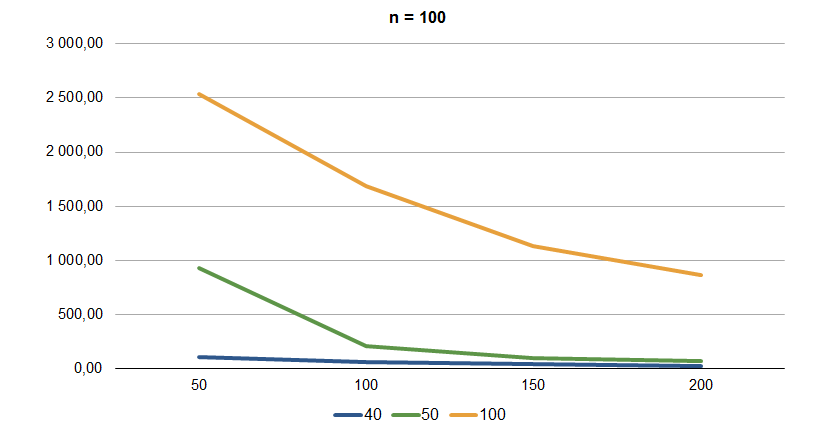
\includegraphics[scale = 0.7]{img/GA_diff_100.PNG}
         \caption{Diff, $n = 100$}
  \end{center}
\end{figure}

\newpage
\subsection{Średnia różnica dla zmiennego \textit{k} i stałego \textit{n = 1000}}
\paragraph{}
\begin{center}
    \begin{longtable}{|c|c|c|c|c|}
        \hline
        \backslashbox{$k$}{$m$} & 40 & 50 & 100\\ \hline
        50 & 10,99 & 14,33 & 378,84 \\ \hline
        100 & 2,59 & 9,17 & 87,50 \\ \hline
        150 & 2,53 & 2,14 & 46,63 \\ \hline
        200 & 1,44 & 48,89 & 39,68 \\ \hline
        \caption{Diff, $n = 1000$}
    \end{longtable}
\end{center}

\begin{figure}[htbp]
  \begin{center}
         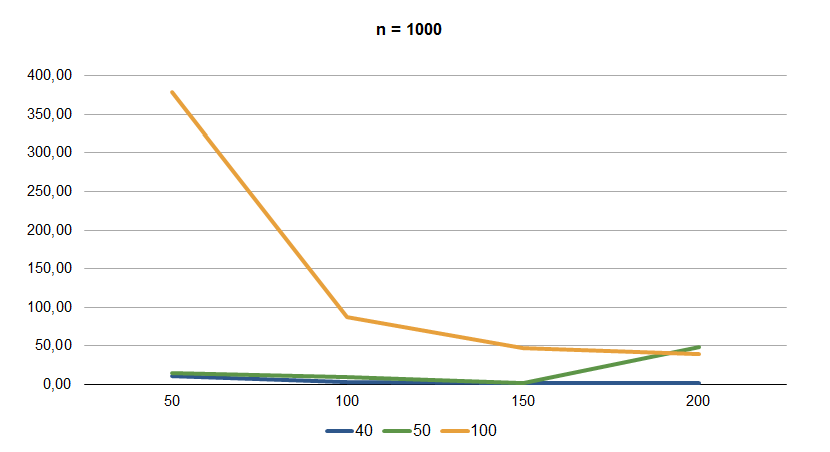
\includegraphics[scale = 0.7]{img/GA_diff_1000.PNG}
         \caption{Diff, $n = 1000$}
  \end{center}
\end{figure}

\newpage
\subsection{Średnia czas rozwiązywania dla zmiennego \textit{k} i stałego \textit{n = 100}}
\begin{center}
    \begin{longtable}{|c|c|c|c|}
        \hline
        \backslashbox{$k$}{$m$} & 40 & 50 & 100\\ \hline
            50 & 136,45 & 219,75 & 497,38\\ \hline
            100 & 261,98 & 391,01 & 918,89\\ \hline
            150 & 409,40 & 598,76 & 1 394,21\\ \hline
            200 & 572,62 & 908,32 & 1 847,48\\ \hline

        \caption{Time, $n = 100$}
    \end{longtable}
\end{center}

\begin{figure}[htbp]
  \begin{center}
         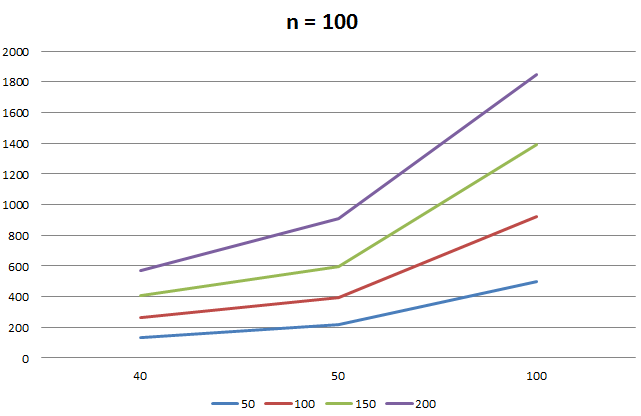
\includegraphics[scale = 0.7]{img/GA_n_100.PNG}
         \caption{Time, $n = 100$}
  \end{center}
\end{figure}


\newpage
\subsection{Średnia czas rozwiązywania dla zmiennego \textit{k} i stałego \textit{n = 1000}}
\begin{center}
    \begin{longtable}{|c|c|c|c|}
        \hline
        \backslashbox{$k$}{$m$} & 40 & 50 & 100\\ \hline
            50 & 1 285,72 & 1 904,94 & 4 428,43\\ \hline
            100 & 2 492,99 & 3 706,92 & 9 026,62\\ \hline
            150 & 3 713,95 & 5 595,20 & 13 981,76\\ \hline
            200 & 4 954,24 & 7 452,48 & 18 717,00\\
        \hline
        \caption{Time, $n = 1000$}
    \end{longtable}

\end{center}

\begin{figure}[htbp]
  \begin{center}
         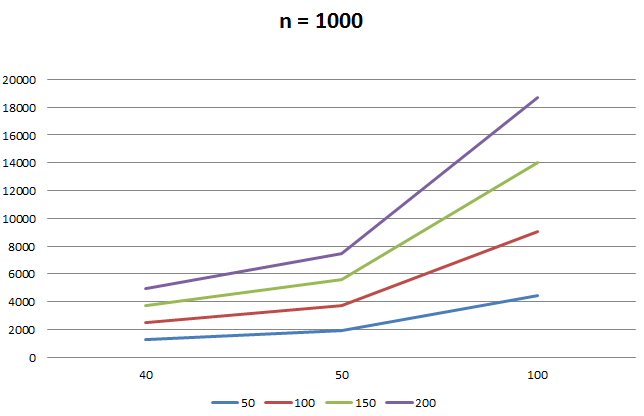
\includegraphics[scale = 0.7]{img/GA_n_1000.PNG}
         \caption{Time, $n = 1000$}
  \end{center}
\end{figure}


\newpage

\section{Wnioski}
\paragraph{}
Po przeprowadzeniu analizy wyników testów, jednoznacznie widać, że rozmiar instancji ma znaczący wpływ na czas działania algorytmu. Znaczną część czasu wykonywania algorytmu zajmuje obliczanie funkcji kosztu, której czas jest zależny od rozmiaru instancji. Głównym parametrem, od którego zależna jest dokładność wyniku, a co za tym idzie czas dochodzenia do rozwiązania jest parametr $n$, określający ilość iteracji. Ważnym parametrem jest również $k$ - wielkość populacji. Odpowiednio dobrane parametry wraz z czynnikiem losowym (mutacja) pozwalają uzyskać zadowalające wyniki.

\paragraph{}
Algorytm genetyczny pozwala na znalezienie przybliżonego rozwiązania problemu $sNPh$. Wiąże się to jednak z koniecznością dobrania odpowiednich parametrów, co nie jest zadaniem łatwym, a także z wybraniem odpowiedniego sposobu krzyżowania populacji. W miarę poprawy wyników poprzez dobierane parametry, wzrasta czas wykonania algorytmu. W celu obliczenia problemu, musimy odpowiedzieć sobie na pytanie, jak dokładne rozwiązanie nas interesuje i ile czasu możemy na nie poświęcić.

\newpage
\section{Porównanie}
\paragraph{} % (fold)
\label{par:}
\subsection{Porównanie średniego czasu algorytmów}
\begin{center}
    \begin{longtable}{|c|c|c|c|}
        \hline
        Alg & 40 & 50 & 100 \\ \hline
        G(k=50, n=100) & 136,45 & 219,75 & 497,38\\ \hline
        G(k=100, n=100)& 261,98 & 391,01 & 918,89\\ \hline
        G(k=150, n=100)& 409,40 &  598,76 & 1 394,21\\ \hline
        G(k=200, n=100)& 572,62 & 908,32 & 1 847,48\\ \hline
        G(k=50, n=1000)& 1 285,72& 1 904,94& 4 428,43\\ \hline
        G(k=100, n=1000)  &  2 492,99 &3 706,92& 9 026,62\\ \hline
        G(k=150, n=1000)   & 3 713,95 &5 595,2  &13 981,76\\ \hline
        G(k=200, n=1000)   & 4 954,24& 7 452,48& 18 717,00\\ \hline
        TS(n=10, k=4, t=7) & 23,11 &  46,81 &  333,83\\ \hline
        TS(n=10, k=5, t=7) & 25,96 &  50,96 &  368,84\\ \hline
        TS(n=10, k=6, t=7) & 26,23 &  39,14 &  327,85\\ \hline
        TS(n=10, k=7, t=7) & 19,42  & 38,48  & 314,94\\ \hline
        TS(n=100, k=4, t=7)& 188,06 & 378,68 & 3 028,87\\ \hline
        TS(n=100, k=5, t=7)& 208,98 & 375,12 & 3 009,74\\ \hline
        TS(n=100, k=6, t=7)& 206,57 & 382,79 & 3 004,64\\ \hline
        TS(n=100, k=7, t=7) &185,13  &387,76 & 3 003,10\\ \hline
        SA(0,990000)  &  1,89  &  2,01 &   3,09\\ \hline
        SA(0,999000)  &  15,88 &  18,74 &  30,36\\ \hline
        SA(0,999900)  &  167,36 & 189,63 & 305,09\\ \hline
                \caption{Średni czas}
    \end{longtable}

\end{center}

\begin{landscape}
\begin{figure}[htbp]
  \begin{center}
         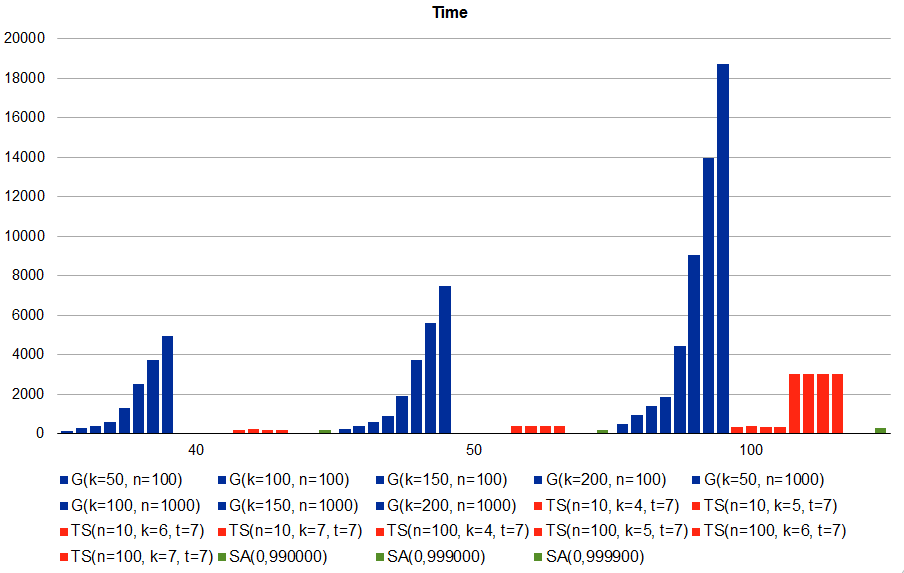
\includegraphics[scale = 1.0]{img/timeAll.PNG}
         \caption{Średni czas}
  \end{center}
\end{figure}
\end{landscape}


\subsection{Porównanie różnicy wyników algorytmów}
\begin{center}
    \begin{longtable}{|c|c|c|c|}
        \hline
         Alg  & 40&  50 & 100 \\ \hline
        GA(k=50, n=100)& 108,04&  928,76 & 2 535,24\\ \hline
        GA(k=100, n=100)  &  57,86 &  212,16 & 1 682,69\\ \hline
        GA(k=150, n=100)  &  38,76  & 92,89&   1 133,71\\ \hline
        GA(k=200, n=100)   & 26,19  & 69,96 &  859,94\\ \hline
        GA(k=50, n=1000)   & 10,99 &  14,33 &  378,84\\ \hline
        GA(k=100, n=1000) & 2,59  &  9,17  &  87,50\\ \hline
        GA(k=150, n=1000) &  2,53  &  2,14 &   46,63\\ \hline
        GA(k=200, n=1000)  & 1,44   & 48,89&   39,68\\ \hline
        TS(n=10, k=4, t=7) & 89,35  & 356,44 & 1 170,06\\ \hline
        TS(n=10, k=5, t=7) & 89,35  & 356,44&  1 170,06\\ \hline
        TS(n=10, k=6, t=7) & 89,35 &  356,44&  1 170,06\\ \hline
        TS(n=10, k=7, t=7) & 89,35 &  356,44 & 1 170,06\\ \hline
        TS(n=100, k=4, t=7) &1,50 &   2,21 &   28,78\\ \hline
        TS(n=100, k=5, t=7) &1,31  &  1,69 &   30,62\\ \hline
        TS(n=100, k=6, t=7)& 1,33 &  6,41  &  33,63\\ \hline
        TS(n=100, k=7, t=7) &1,78  & 2,43  &  33,78\\ \hline
        SA(0,990000)  &  8,07   & 15,77 &  337,97\\ \hline
        SA(0,999000)  &  0,16  &  0,55  &  9,93\\ \hline
        SA(0,999900)  &  0,11  &  0,01 &   0,57\\ \hline
                \caption{Różnica}
    \end{longtable}

\end{center}

\begin{landscape}
\begin{figure}[htbp]
  \begin{center}
         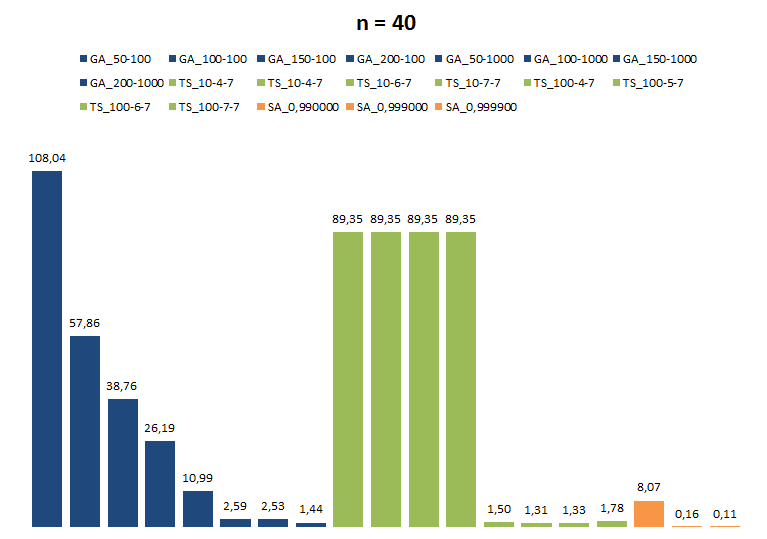
\includegraphics[scale = 1.0]{img/all40.PNG}
         \caption{40 zadań}
  \end{center}
\end{figure}
\end{landscape}

\begin{landscape}
\begin{figure}[htbp]
  \begin{center}
         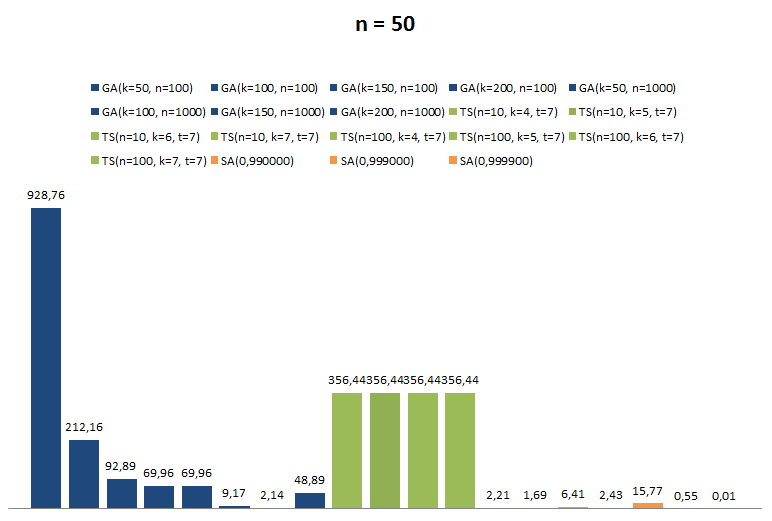
\includegraphics[scale = 1.0]{img/all50.PNG}
         \caption{50 zadań}
  \end{center}
\end{figure}
\end{landscape}

\begin{landscape}
\begin{figure}[htbp]
  \begin{center}
         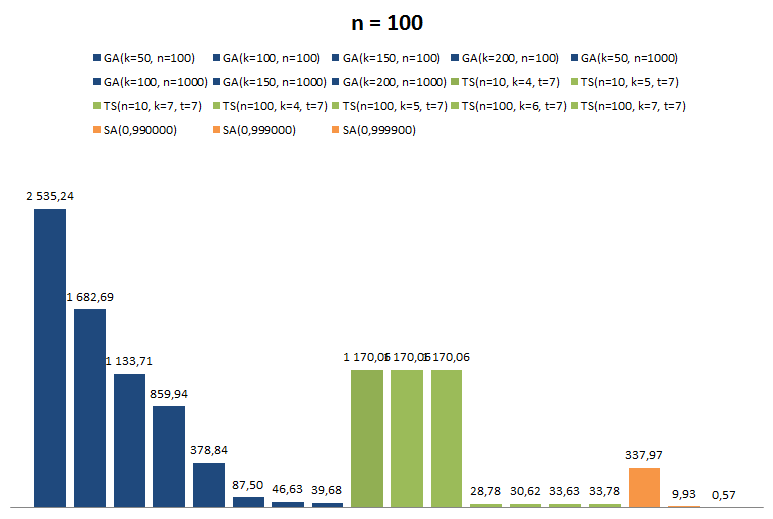
\includegraphics[scale = 1.0]{img/all100.PNG}
         \caption{100 zadań}
  \end{center}
\end{figure}
\end{landscape}
\end{document}



